\documentclass[tikz,border=2mm]{standalone}
\usepackage{enumitem}
\usepackage{stmaryrd} 
\usepackage{amsfonts}
\usepackage{amsthm}
\usepackage{amssymb}
\usepackage{amsmath}
\usepackage{hyperref}
\usepackage{tikz}
\usetikzlibrary{arrows.meta, positioning} % optional: arrows & positioning

\begin{document}
    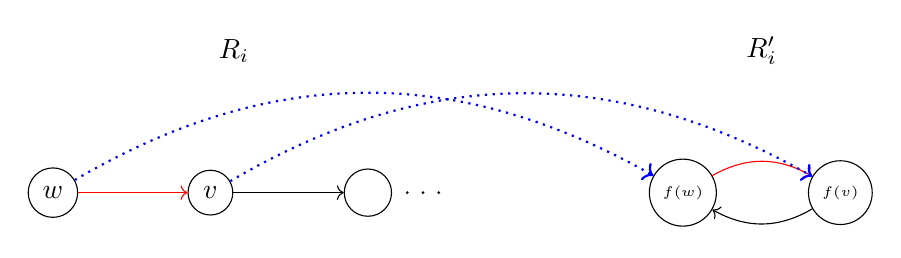
\begin{tikzpicture}
        % nodes
        \node[draw, circle, minimum size=0.2cm](A) at (0,0) {$w$};
        \node[draw, circle, minimum size=0.2cm] (B) at (2,0) {$v$};
        \node[draw, circle, minimum size=0.6cm] (C) at (4,0) {};
        \filldraw (4.5,0) circle (0.01cm);
        \filldraw (4.7,0) circle (0.01cm);
        \filldraw (4.9,0) circle (0.01cm);
        \node at (2.3,1.8) {$R_i$};
        \node at (9,1.8) {$R_i'$};

        % edges
        \draw [->,red] (A) -- (B);
        \draw [->] (B) -- (C);

        \node[draw, circle, font=\tiny\itshape]  (D) at (8,0) {$f(w)$};
        \node[draw, circle, font=\tiny\itshape] (E) at (10,0) {$f(v)$};

        \draw[->,red, bend left=30] (D) to (E);
        \draw[->, bend left=30] (E) to (D);

        \draw[->, dotted, blue, bend left=30, thick] (A) to (D);
        \draw[->, dotted, blue, bend left=30,thick] (B) to (E);



    \end{tikzpicture}

\end{document}